\documentclass[UTF8,a4paper]{ctexart}
\usepackage[margin=1in]{geometry}
\usepackage{graphicx,float,array,color}
\author{qhy}
\date{\today}
\title{ML Note}
\begin{document}
    \maketitle
    \tableofcontents
    \newpage
    \section{SVM}
    定义标签:$\hat{y} = \{+1,-1\}$,+1表示正类,-1表示负类
    定义输出:
    \begin{equation}
        g(x) = \left \{
            \begin{array}{ll}
                +1 & ,f(x) > 0 \\
                -1  & ,f(x) >0
            \end{array} \right .
    \end{equation}

    定义loss functon:
    \begin{equation}
        L(f) = \sum_n I(g(x^n \neq \hat{y}^n))
    \end{equation}

    也就是统计分类错误的个数,从更一般的角度来看,就是每分类错误一个,就给一定的惩罚

    分析:$\hat{y^n}f(x^n)>0$的时候,分类正确,无论是正类还是负类,

    如果把这个看做一个新的变量t,那么损失函数(一个数据的损失函数)就可以定义成$t>0$时无惩罚,$t<0$的时候给出一定的惩罚。

    \begin{figure}[H]
        \centering
        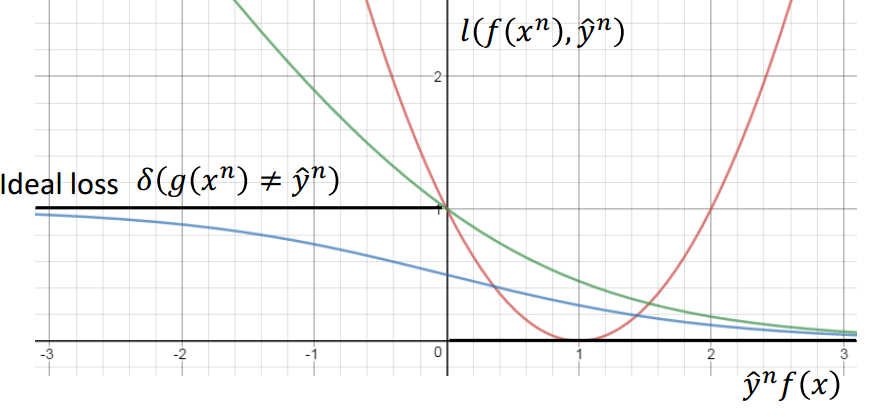
\includegraphics[scale = 0.3]{assets/ML_1a136.png}
        \label{figlossfunction}
    \end{figure}

    理想的情况就是图\ref{figlossfunction}中的黑线,分类错误就给出惩罚。

    由于此loss function使用梯度下降算法麻烦,故使用一个惩罚函数l代替I:
    \begin{equation}
        L(f) = \sum_n I(f(x^n , \hat y^n))
    \end{equation}

    红色线为\textbf{Square loss}:
    \begin{equation}
        l(f(x^n , \hat y^n) = (\hat y^n f(x^n) - 1)^2
    \end{equation}
    显然是不合理的,因为它对于分类正确的结果也给出了惩罚。

    蓝色线为\textbf{sigmoid+ square loss}:
    \begin{equation}
        l(f(x^n , \hat y^n) = (\sigma(\hat y^n f(x^n)) - 1)^2
    \end{equation}
    这样,得到的结果是合理的,对于分类正确,确定性高的给出低惩罚,对于分类错误,甚至错误的离谱的,则给出大的惩罚

    但是有一个问题就是,对于分类错误的结果,它的惩罚很低。

    绿色线为\textbf{Sigmoid + cross entropy}
    \begin{equation}
        l(f(x^n , \hat y^n) = \ln(1 + exp(-y^n f(x^n)))
    \end{equation}

    蓝色线为\textbf{hinge loss}:
    \begin{equation}
        l(f(x^n , \hat y^n) = max(0, 1 - y^n f(x^n))
    \end{equation}

    对于分类正确的结果,只要$yf(x) < 1$的数据还是会给出惩罚,而SVM采用的就是$Hinge Loss$

    从$f(x)$来看,$f(x)$为分界线,只要在$f(x)$上下距离为1的样本都会给出惩罚。

        \subsection{线性SVM}
        模型如下:
        \begin{figure}[H]
            \centering
            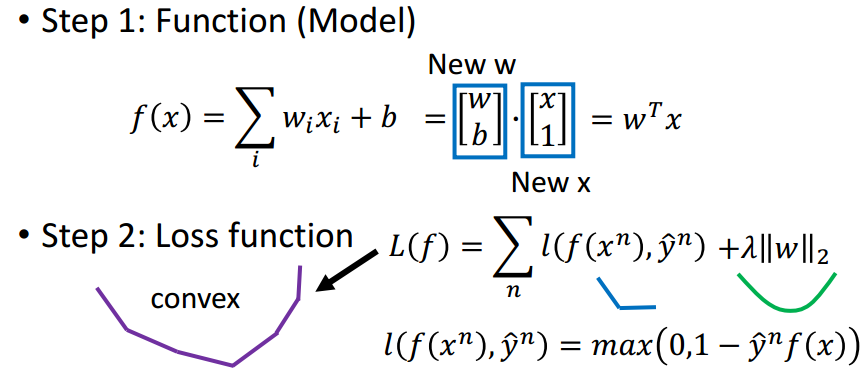
\includegraphics[scale = 0.3]{assets/ML_2f26e.png}
            \label{figlinearSVM}
        \end{figure}

        梯度下降:
        \begin{figure}[H]
            \centering
            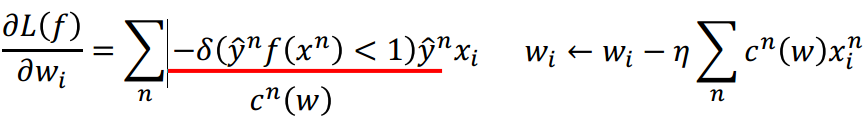
\includegraphics[scale = 0.3]{assets/ML_b932f.png}
            \label{figlinearSVMGradientDescent}
        \end{figure}

        \subsection{线性SVM2}
        {\color{red} 至此,线性SVM结束,但是这个SVM和之前见到的SVM貌似不太一样?对偶问题,SMO,等等这些东东呢?}

        另一种描述:
        \begin{figure}[H]
            \centering
            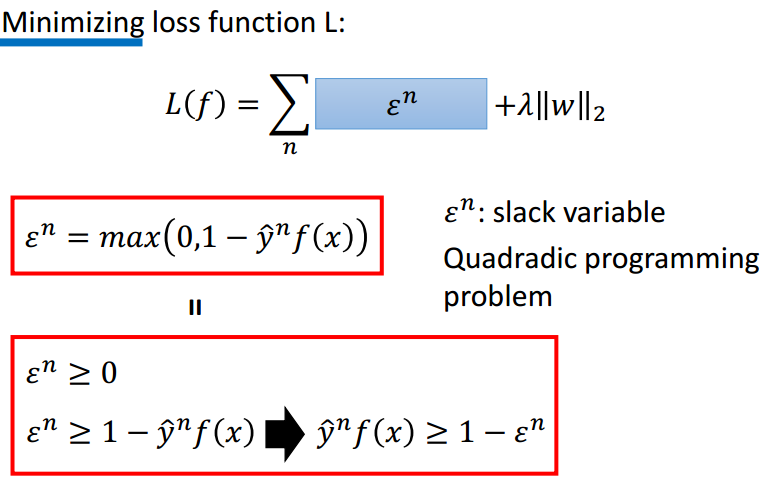
\includegraphics[scale = 0.3]{assets/ML_e1a0b.png}
        \end{figure}

        经过这样处理,原问题从
        最小化:
        \begin{figure}[H]
            \centering
            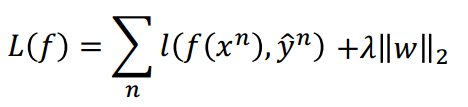
\includegraphics[scale = 0.3]{assets/ML_5215d.png}
        \end{figure}

        变成了最小化:
        \begin{figure}[H]
            \centering
            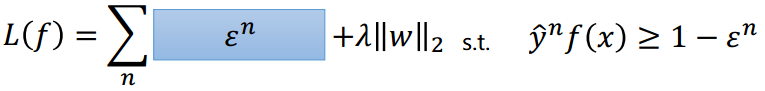
\includegraphics[scale = 0.3]{assets/ML_a74a0.png}
        \end{figure}

        进一步处理,问题变成最小化:
        \begin{figure}[H]
            \centering
            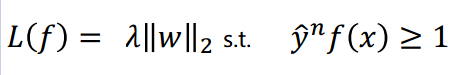
\includegraphics[scale = 0.3]{assets/ML_371e4.png}
        \end{figure}

        \subsection{Kernel SVM}
        简单地从梯度下降的角度来看,那么最终得到的$w^*$一定是所有$x_i$的线性组合,i.e.
        \begin{equation}
            w^* = \sum_i a_i^* x_i
        \end{equation}

        而由于使用\textbf{hinge loss}的原因,大部分的$a_i^* = 0$,对于$a_i^* \neq 0$的$x_i$,则称为\textbf{Support Vector}

        那么最终的解的形式变成了$f(x) = \sum_i a_i(x_i\cdot x)$

         若引入核函数,则是$f(x) = \sum_i a_i\cdot K(x_i\cdot x)$

        而这个解的形式,则可以看成是一个单隐层神经网络:

        \begin{figure}[H]
            \centering
            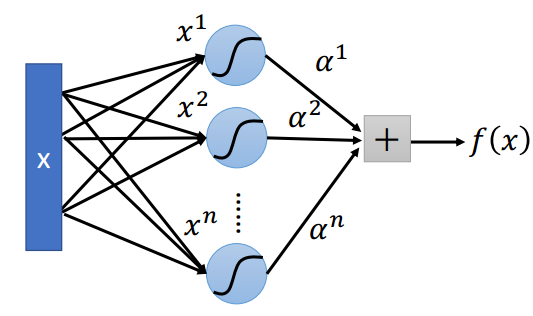
\includegraphics[scale = 0.3]{assets/ML_b1b86.png}
        \end{figure}

        其中,每一个\textbf{Support Vector}表示一个神经元。

        {\color{blue} 这里为了引入核函数,把问题变成了这种形式,参数变成了$a$,但一样可以用,梯度下降去解决,

        从这里来看,应该是由$a$决定哪些是 \textbf{支持向量},而不是由支持向量,决定哪些$a = 0$}

        \textbf{为什么说RBF是对应的是无穷为的点积?}

        因为RBF使用泰勒展开之后,有无穷项,每一项代表若干个维度的分量分别相乘之和的结果。

        \textbf{怎么设计核函数?}
        满足 mercer 条件的任一函数都可以是核函数。

        {\color{red}}

        \subsection{SVM的应用与变种}
        \begin{itemize}
            \item SVR
            \item Ranking SVM
            \item one-class SVM
            \item Recursive Kernel
        \end{itemize}

    \section{Structure Learning}
    之前我们接触的大部分都是输入是一个向量,输出是一个实数
    但如果我们要输出一个序列则怎么处理?

    这里有一个大致的框架:\\
    设$X$是输入,$Y$是输出,$F(X,Y)$描述X,Y的相似度,或者是X输出Y的概率\\
    对于训练过程,我们要做的就是最大化训练样本输入和输出的相似度,i.e.
    \begin{equation}
        \max F(X,Y)
    \end{equation}

    对于测试过程,我们的输出就是在$Y$的空间中,与测试输入$X$,$F(X,Y)$最大的那个$Y$

    那么,就有3个问题需要解决:
    \begin{itemize}
        \item [1. ] $F(X,Y)$是什么样子?
        \item [2. ] 怎么有效快速地输出y?
        \item [3. ] 怎么训练?
    \end{itemize}

    {\color{blue} 总的来说,就是把X和Y两个不同的东西,表示在同一个空间内,这样才能建立起度量,进而才有优化的方向。}

    {\color{blue} 这三个问题和 HMM中的三个问题是一致的,因为HMM就是Structure Learning中的一种}

        \subsection{Structured Liner Model}
        F(x,y)的形式:y可以看成是x在特征空间中的投影,我们要做的就是在特征空间中的点距离y尽可能地近,或者是相似度尽可能大。
        \begin{figure}[H]
            \centering
            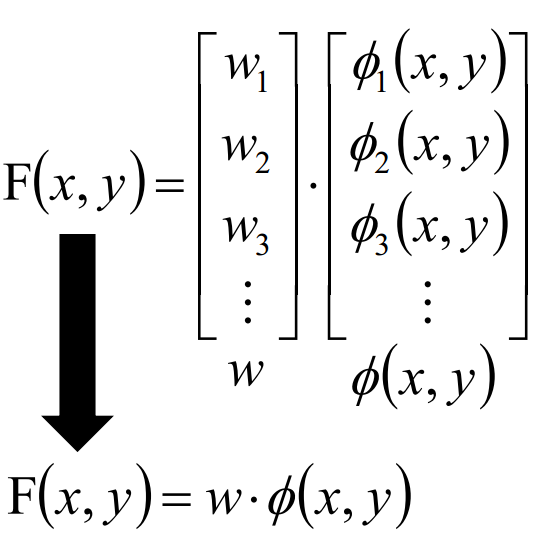
\includegraphics[scale = 0.3]{assets/ML_eca3e.png}
        \end{figure}

        我们可以简单地定义损失函数就是$F(x,\hat{y}) - F(x,d\dot y)$,也就是当前预测的点到目标点的距离。

        其中$\dot y$是$F{x,y}$最大的$y$,我们只需要考虑最大的$y$即可,而不需要考虑其他。

        至此,我们就可以用梯度下降的方法进行训练:
        \begin{figure}[H]
            \centering
            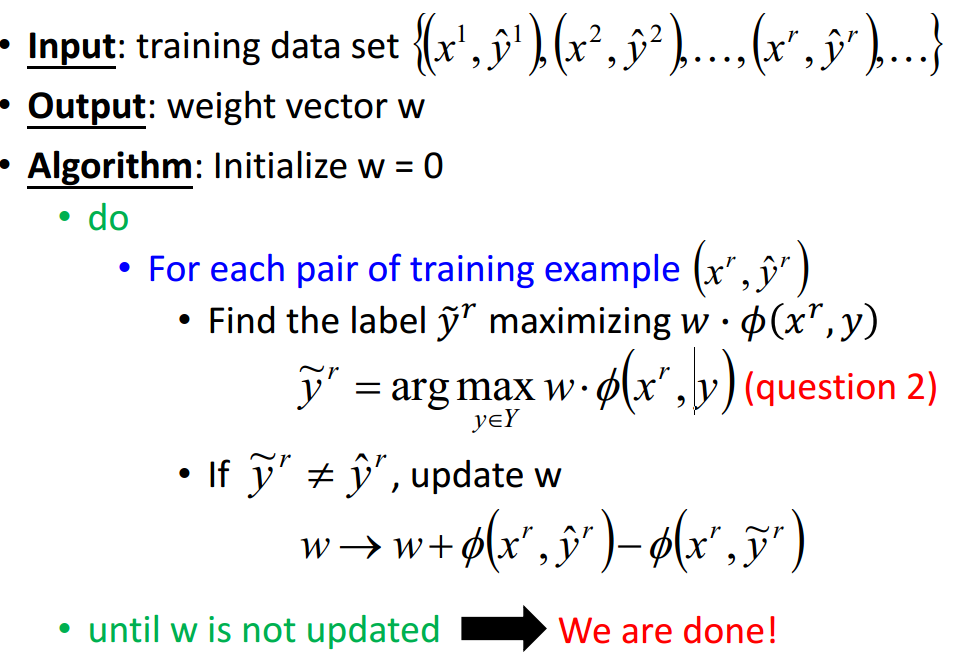
\includegraphics[scale = 0.3]{assets/ML_7db22.png}
        \end{figure}

        \textbf{收敛性证明}:对于线性可分的数据,我们可以证明,最多需要$(\frac{R}{\delta})^2$次迭代就可以收敛。

        其中,$R$表示特征空间中任意两个y之间的最大距离,$\delta$表示margin

        也就是说,迭代的次数和样本的规模无关。

        \begin{figure}[H]
            \centering
            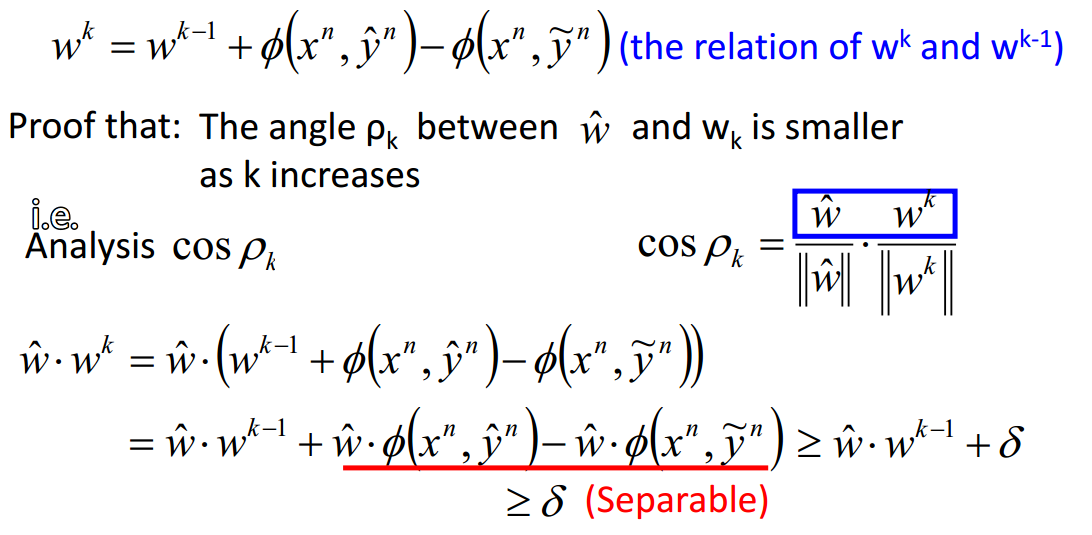
\includegraphics[scale = 0.3]{assets/ML_178a9.png}
        \end{figure}
        即,我们要证明,随着迭代的过程,w是不断向最优解靠近的,也就是夹角不断变小

        \begin{figure}[H]
            \centering
            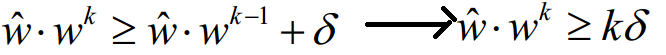
\includegraphics[scale = 0.3]{assets/ML_85362.png}
        \end{figure}


        \begin{figure}[H]
            \centering
            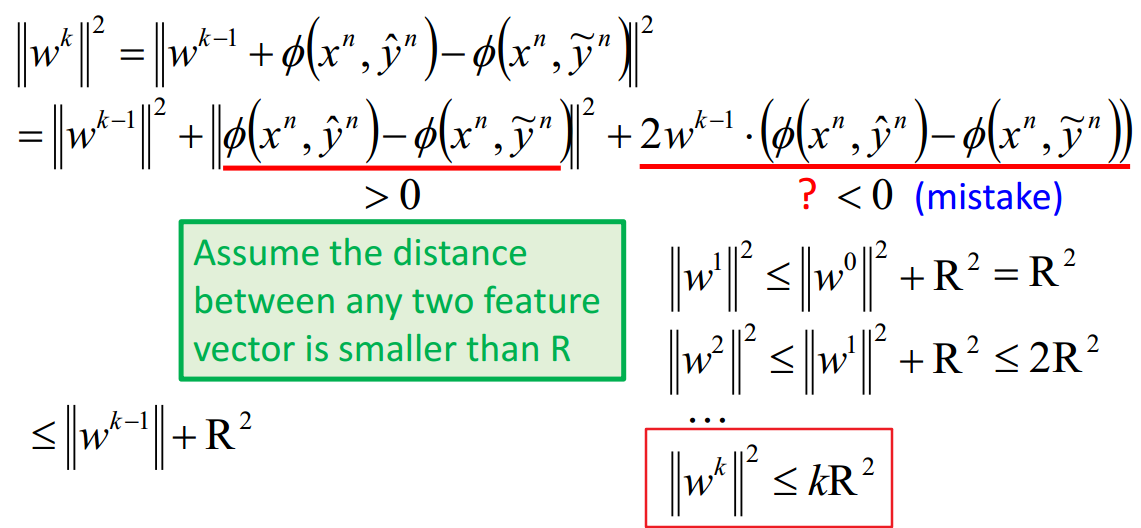
\includegraphics[scale = 0.3]{assets/ML_2532d.png}
        \end{figure}

        \begin{figure}[H]
            \centering
            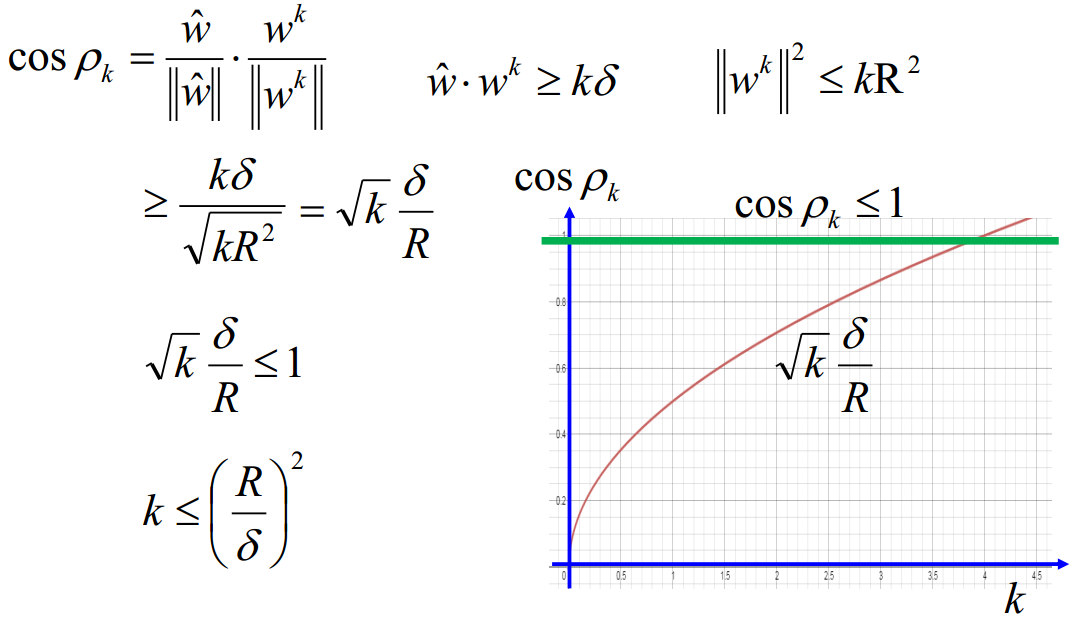
\includegraphics[scale = 0.3]{assets/ML_78f61.png}
        \end{figure}

        {\color{blue}
        这里我们并没有证明$\cos \rho$是增大到1的,我们证明的是它的一个下界是不断增大到1,那么根据夹逼定理得证。

        值得注意的是,这里有一个参数$\delta$,这个需要事先人为设定,当约束比较严格的是,则迭代次数较多,当约束比较松的时候,则迭代次数少。

        $\delta$:对于这个参数的理解,我们并不要求整个算法的输入$X$在特征空间中的表示一定要和$Y$的表示重合,只要它们的差值在一定的范围内都是可接受的,因此,这个参数也叫margin
        }



















\end{document}
